\section{Measuring money in circulation}
\label{sec:measure}%

In \cite{pernice2019cryptocurrencies} monetary units are seen as ``in circulation'' for measurement day \(\perd\)
if they have been used as a medium of exchange. %
Money is referred to as circulating if it has been moved economically within the last day, month, year or generally any time period $\wndw_\perd$%
The measure is set up in a way that measurement-day \(\perd\) constitutes the last day of window \(\wndw_\perd\) for which money in circulation is to be estimated (compare figure~\ref{fig:timevars}). %
Monetary units brought into circulation in the last second of day \(\perd\) are to be attributed to belong to money in circulation for \(\perd\). %  

\begin{figure*}[ht!]%
	\centering
	\ifdefined\varInputFigs%
%	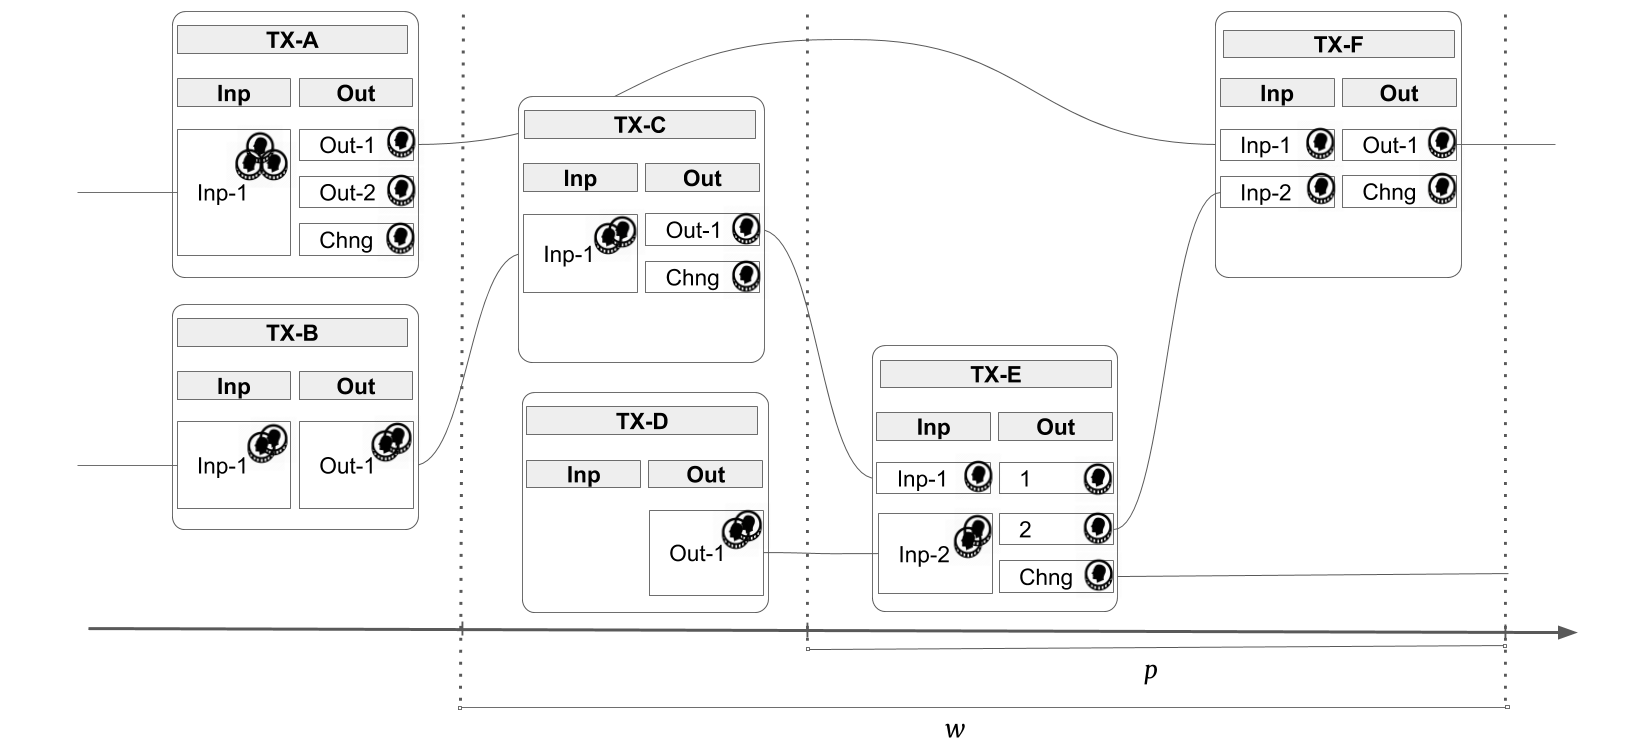
\includegraphics[width=0.8\linewidth]{fig/mcirc_concept_window_uneqal_period_HR}%
	%-------------------------------------------------------------------------------
\usetikzlibrary{calc}
%coordinate test point. Use as follows: 	\coordinate (cen) 	 	 at (0,0) (cen) [point];
\tikzset{
	every point/.style = {radius={\pgflinewidth}, opacity=1, draw, solid, fill=white},
	pt/.pic = {
		\begin{pgfonlayer}{foreground}
			\path[every point, #1] circle;
		\end{pgfonlayer}
	},
	point/.style={insert path={pic{pt={#1}}}}, point/.default={},
	point name/.style = {insert path={coordinate (#1)}}
}
%-------------------------------------------------------------------------------

% basic delacations
\pgfdeclarelayer{background}%
\pgfdeclarelayer{foreground}%
\pgfsetlayers{background,main,foreground}%

%Coin Symbol--------------------------------------------------------------------
\tikzset{%
	pics/coin/.style n args={3}{%
		code ={
			\def \coinLineWidth {#1}%
			\def \coinCenDist   {#2}%
			\def \circRad       {#3}%
			\def \signRad       {\circRad*0.20}%
			\def \signRadProp   {0.45}
			\def \signRadExt    {\signRad*\signRadProp}
			\def \signRadOut    {\signRad+\signRadExt}
			\def \signAngle     {30}
			\def \sinSignAngle  {sin(\signAngle)}
			\def \cosSignAngle  {cos(\signAngle)}
			\def \signWidth     {{pow((pow(\signRadOut,2)-pow(\sinSignAngle*\signRad,2)),0.5)-(\cosSignAngle)*\signRad)}}
			
			\def \startIX       {{cos(\signAngle)*\signRad}}
			\def \startIY       {{\sinSignAngle*\signRad}}
			
			\def \startOY       {\startIY}
			\def \signAngleOutS {{atan((\sinSignAngle*\signRad)/pow((pow(\signRadOut,2)-pow(\sinSignAngle*\signRad,2)),0.5))}}
			\def \signAngleOutE {{360-atan((\sinSignAngle*\signRad)/pow((pow(\signRadOut,2)-pow(\sinSignAngle*\signRad,2)),0.5))}}
	%
			\coordinate ()          at ( 0.0     , 0.0);%
			\coordinate (cen)       at ( 0.0     , 0.0);%
			\coordinate (cenB)      at ($(cen)    + ( 0.00,-\coinCenDist)$);%
						
			\node[
				circle,
				draw = black,
				fill = white,
				line width = \coinLineWidth,
				minimum size = \circRad,
				inner sep = 0pt,
				outer sep = 0pt,
			](NCD) at (cenB) {};
			
			\node[
				circle,
				draw = black,
				fill = white,
				line width = \coinLineWidth,
				minimum size = \circRad,
				inner sep = 0pt,
				outer sep = 0pt,
			](NCU) at (cen) {};
			
%			\draw[ - , line width = \coinLineWidth, black] (NCU.195) -- (NCD.195);
			\draw[-, line width = \coinLineWidth, black] (NCU.210) -- (NCD.210);
			\draw[-, line width = \coinLineWidth, black] (NCU.225) -- (NCD.225);
			\draw[-, line width = \coinLineWidth, black] (NCU.240) -- (NCD.240);
			\draw[-, line width = \coinLineWidth, black] (NCU.255) -- (NCD.255);
			\draw[-, line width = \coinLineWidth, black] (NCU.270) -- (NCD.270);
			\draw[-, line width = \coinLineWidth, black] (NCU.285) -- (NCD.285);
			\draw[-, line width = \coinLineWidth, black] (NCU.300) -- (NCD.300);
			\draw[-, line width = \coinLineWidth, black] (NCU.315) -- (NCD.315);
			\draw[-, line width = \coinLineWidth, black] (NCU.330) -- (NCD.330);
%			\draw[ - , line width = \coinLineWidth, black] (NCU.345) -- (NCD.345);
			
			\draw[
				 - ,
				 line width = \coinLineWidth,
				 black!80!white,
				 fill = black!80!white
			]
				(\startIX,-\startIY) arc (360-\signAngle:\signAngle:\signRad)
				-- +(\signWidth, 0.0)
				arc (\signAngleOutS:\signAngleOutE:\signRadOut)
				-- (\startIX,-\startIY)
				-- cycle
				;
		}%
		
	} ,%
	pics/coin/.default={1.0pt}{0.1}{1cm}%
}%
%
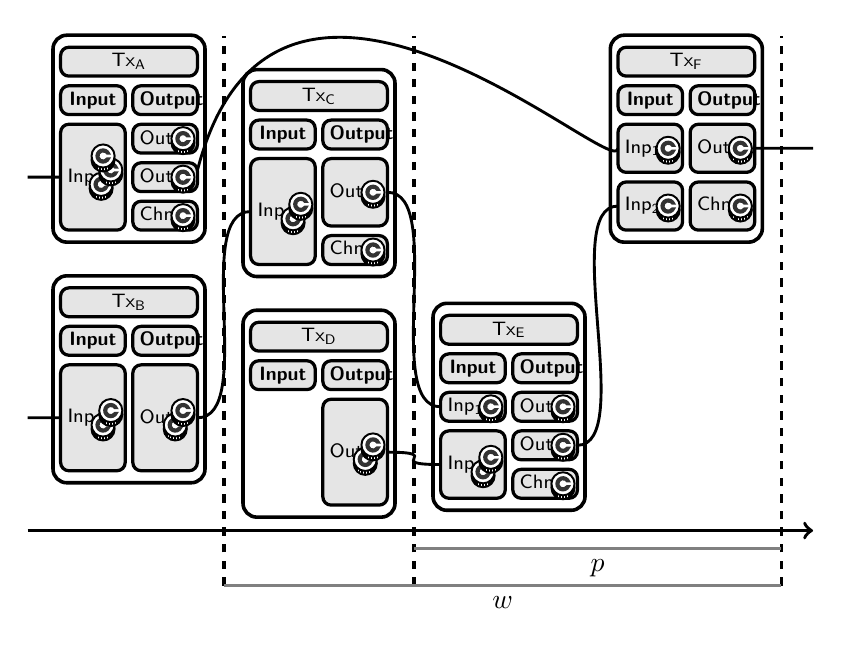
\begin{tikzpicture}
	\def \debugPoint   {}%
%b	\def \debugPoint   {point}%
	% font settings ############################################################
	\def \fontset      {\scriptsize\sffamily}
	% color definition #########################################################
	\def \colorOut     {black!100!white}
	\def \colorIn      {black!10!white}
	% arrow and line definitions ###############################################
	\def \lineW        {1.3pt}
	% width/height definition ##################################################
	\def \picW         {\linewidth*25.5/31}%
	\def \picH         {\paperheight*7.75/31}%
	\def \TH           {\picH*0.4}%picH*0.5*0.8
	
	\def \WBA          {\picW*11.50/31}
	\def \WLA          {\picW* 7.75/31}
	\def \WBB          {\picW* 4.00/31}
	\def \WLB          {\picW* 0.25/31}
	\def \WBC          {\picW* 3.50/31}
	\def \WBD          {\picW*10.50/31}
	\def \WLD          {\picW*14.25/31}
	% width/height nodes/boxes###################################################
	\def \BOH          {\picH* 0.35  }
	\def \BOW          {\picW* 6.0/31}
	
	% node positioning
	\def \BIPX         {\BOW*0.2375}
	
	% tikz styles################################################################
	\tikzstyle{lineIO} = [
		- ,
		line width = \lineW*0.8,
	]
	\tikzstyle{nodeOuter}   = [
		draw,
		rectangle,
		rounded corners=5pt,
		solid,
		line width = \lineW,
		black,
		inner sep = 0pt,
		outer sep = 0pt,
		text width = \BOW,
		minimum width = \BOW,
		minimum height = \BOH*1.075,
	]
	\tikzstyle{nodeInner}   = [
		draw,
		rectangle,
		rounded corners=3pt,
		solid,
		line width = \lineW*0.9,
		black,
		fill = \colorIn,
		inner sep = 0pt,
		outer sep = 0pt,
	]
	\tikzstyle{nodeInnerA}  = [
		nodeInner,
		align = center,
		text width = \BOW*0.9-3pt,
		minimum width = \BOW*0.9,
		minimum height = \BOH*0.15,
	]
	\tikzstyle{nodeInnerB}  = [
		nodeInner,
		align = left,
		text width = \BOW*0.425-5pt,
		minimum width = \BOW*0.425,
	]
	\tikzstyle{nodeInnerBA} = [
		nodeInnerB,
		minimum height = \BOH*0.15,
	]	
	\tikzstyle{nodeInnerBAC}b= [
		nodeInnerB,
		minimum height = \BOH*0.15,
		align = center,
	]
	\tikzstyle{nodeInnerBB} = [
		nodeInnerB,
		minimum height = \BOH*0.25,
	]
	\tikzstyle{nodeInnerBC} = [
		nodeInnerB,
		minimum height = \BOH*0.35,
	]
	\tikzstyle{nodeInnerBD} = [
		nodeInnerB,
		minimum height = \BOH*0.55,
	]
	% coordinates ###############################################################
	% 1 | 2 | 3 | 4 | 5 | 6 | 7 | 8 | 9 | 10 | 11 | 12 | 13 | 14 |
	% A | B | C | D | E | F | G | H | I |  J |  K |  L |  M |  N |
	
	\coordinate (cen)       at ($(0.0,0.0)   + ( 0.0       , 0.0         )$) (cen)   [\debugPoint];%
	
	\coordinate (PLU)       at ($(cen)       + (-\picW*0.5 , \picH*0.5   )$) (PLU)   [\debugPoint];%
	\coordinate (PLD)       at ($(cen)       + (-\picW*0.5 ,-\picH*0.5   )$) (PLD)   [\debugPoint];%
	\coordinate (PRU)       at ($(cen)       + ( \picW*0.5 , \picH*0.5   )$) (PRU)   [\debugPoint];%
	\coordinate (PRD)       at ($(cen)       + ( \picW*0.5 ,-\picH*0.5   )$) (PRD)   [\debugPoint];%
	
	
	\coordinate (TC)        at ($(cen)       + ( 0.0       ,-\TH         )$) (TC)    [\debugPoint];%
	\coordinate (TL)        at ($(TC)        + (-\picW*0.5 , 0.0         )$) (TL)    [\debugPoint];%
	\coordinate (TR)        at ($(TC)        + ( \picW*0.5 , 0.0         )$) (TR)    [\debugPoint];%
	
	\coordinate (BAC)       at ($(cen)       + (-\WBA      , 0.0         )$) (BAC)   [\debugPoint];%
	\coordinate (LAC)       at ($(cen)       + (-\WLA      , 0.0         )$) (LAC)   [\debugPoint];%
	\coordinate (BBC)       at ($(cen)       + (-\WBB      , 0.0         )$) (BBC)   [\debugPoint];%
	\coordinate (LBC)       at ($(cen)       + (-\WLB      , 0.0         )$) (LBC)   [\debugPoint];%
	\coordinate (LDC)       at ($(cen)       + ( \WLD      , 0.0         )$) (LDC)   [\debugPoint];%
	\coordinate (BCC)       at ($(cen)       + ( \WBC      , 0.0         )$) (BCC)   [\debugPoint];%
	\coordinate (BDC)       at ($(cen)       + ( \WBD      , 0.0         )$) (BDC)   [\debugPoint];%
	
	\coordinate (LAD)       at ($(LAC)       + ( 0.0       ,-\picH*0.5   )$) (LAD)   [\debugPoint];%
	\coordinate (LAU)       at ($(LAC)       + ( 0.0       , \picH*0.5   )$) (LAU)   [\debugPoint];%
	\coordinate (LBD)       at ($(LBC)       + ( 0.0       ,-\picH*0.5   )$) (LBD)   [\debugPoint];%
	\coordinate (LBDA)      at ($(LBC)       + ( 0.0       ,-\picH*0.4325)$) (LBDA)  [\debugPoint];%
	\coordinate (LBU)       at ($(LBC)       + ( 0.0       , \picH*0.5   )$) (LBU)   [\debugPoint];%
	\coordinate (LCD)       at ($(LDC)       + ( 0.0       ,-\picH*0.5   )$) (LCD)   [\debugPoint];%
	\coordinate (LCDA)      at ($(LDC)       + ( 0.0       ,-\picH*0.4325)$) (LCDA)  [\debugPoint];%
	\coordinate (LCU)       at ($(LDC)       + ( 0.0       , \picH*0.5   )$) (LCU)   [\debugPoint];%
	%coordinates, Box A Down, Tx_B		
	\coordinate (BADCC)     at ($(BAC)       + ( 0.0       ,-\picH*0.125 )$) (BADCC) [\debugPoint];%
	\coordinate (BADCL)     at ($(BADCC)     + (-\BIPX     , 0.0         )$) (BADCL) [\debugPoint];%
	\coordinate (BADCR)     at ($(BADCC)     + ( \BIPX     , 0.0         )$) (BADCR) [\debugPoint];%
	\coordinate (BADAC)     at ($(BADCC)     + ( 0.0       ,-\BOH *0.4   )$) (BADAC) [\debugPoint];%
	\coordinate (BADAL)     at ($(BADAC)     + (-\BIPX     , 0.0         )$) (BADAL) [\debugPoint];%
	\coordinate (BADAR)     at ($(BADAC)     + ( \BIPX     , 0.0         )$) (BADAR) [\debugPoint];%
	\coordinate (BADBC)     at ($(BADCC)     + ( 0.0       ,-\BOH *0.2   )$) (BADBC) [\debugPoint];%
	\coordinate (BADBL)     at ($(BADBC)     + (-\BIPX     , 0.0         )$) (BADBL) [\debugPoint];%
	\coordinate (BADBR)     at ($(BADBC)     + ( \BIPX     , 0.0         )$) (BADBR) [\debugPoint];%
	\coordinate (BADDC)     at ($(BADCC)     + ( 0.0       , \BOH *0.2   )$) (BADDC) [\debugPoint];%
	\coordinate (BADDL)     at ($(BADDC)     + (-\BIPX     , 0.0         )$) (BADDL) [\debugPoint];%
	\coordinate (BADDR)     at ($(BADDC)     + ( \BIPX     , 0.0         )$) (BADDR) [\debugPoint];%
	\coordinate (BADEC)     at ($(BADCC)     + ( 0.0       , \BOH *0.4   )$) (BADEC) [\debugPoint];%	
	%coordinates, Box A Up, Tx_A
	\coordinate (BAUCC)     at ($(BAC)       + ( 0.0       , \picH*0.3125)$) (BAUCC) [\debugPoint];%
	\coordinate (BAUCL)     at ($(BAUCC)     + (-\BIPX     , 0.0         )$) (BAUCL) [\debugPoint];%
	\coordinate (BAUCR)     at ($(BAUCC)     + ( \BIPX     , 0.0         )$) (BAUCR) [\debugPoint];%
	\coordinate (BAUAC)     at ($(BAUCC)     + ( 0.0       ,-\BOH *0.4   )$) (BAUAC) [\debugPoint];%
	\coordinate (BAUAL)     at ($(BAUAC)     + (-\BIPX     , 0.0         )$) (BAUAL) [\debugPoint];%
	\coordinate (BAUAR)     at ($(BAUAC)     + ( \BIPX     , 0.0         )$) (BAUAR) [\debugPoint];%
	\coordinate (BAUBC)     at ($(BAUCC)     + ( 0.0       ,-\BOH *0.2   )$) (BAUBC) [\debugPoint];%
	\coordinate (BAUBL)     at ($(BAUBC)     + (-\BIPX     , 0.0         )$) (BAUBL) [\debugPoint];%
	\coordinate (BAUBR)     at ($(BAUBC)     + ( \BIPX     , 0.0         )$) (BAUBR) [\debugPoint];%
	\coordinate (BAUDC)     at ($(BAUCC)     + ( 0.0       , \BOH *0.2   )$) (BAUDC) [\debugPoint];%
	\coordinate (BAUDL)     at ($(BAUDC)     + (-\BIPX     , 0.0         )$) (BAUDL) [\debugPoint];%
	\coordinate (BAUDR)     at ($(BAUDC)     + ( \BIPX     , 0.0         )$) (BAUDR) [\debugPoint];%
	\coordinate (BAUEC)     at ($(BAUCC)     + ( 0.0       , \BOH *0.4   )$) (BAUEC) [\debugPoint];%
	%coordinates, Box B Down, Tx_D	
	\coordinate (BBDCC)     at ($(BBC)       + ( 0.0       ,-\picH*0.1875)$) (BBDCC) [\debugPoint];%	
	\coordinate (BBDCL)     at ($(BBDCC)     + (-\BIPX     , 0.0         )$) (BBDCL) [\debugPoint];%
	\coordinate (BBDCR)     at ($(BBDCC)     + ( \BIPX     , 0.0         )$) (BBDCR) [\debugPoint];%
	\coordinate (BBDAC)     at ($(BBDCC)     + ( 0.0       ,-\BOH *0.4   )$) (BBDAC) [\debugPoint];%
	\coordinate (BBDAL)     at ($(BBDAC)     + (-\BIPX     , 0.0         )$) (BBDAL) [\debugPoint];%
	\coordinate (BBDAR)     at ($(BBDAC)     + ( \BIPX     , 0.0         )$) (BBDAR) [\debugPoint];%
	\coordinate (BBDBC)     at ($(BBDCC)     + ( 0.0       ,-\BOH *0.2   )$) (BBDBC) [\debugPoint];%
	\coordinate (BBDBL)     at ($(BBDBC)     + (-\BIPX     , 0.0         )$) (BBDBL) [\debugPoint];%
	\coordinate (BBDBR)     at ($(BBDBC)     + ( \BIPX     , 0.0         )$) (BBDBR) [\debugPoint];%
	\coordinate (BBDDC)     at ($(BBDCC)     + ( 0.0       , \BOH *0.2   )$) (BBDDC) [\debugPoint];%
	\coordinate (BBDDL)     at ($(BBDDC)     + (-\BIPX     , 0.0         )$) (BBDDL) [\debugPoint];%
	\coordinate (BBDDR)     at ($(BBDDC)     + ( \BIPX     , 0.0         )$) (BBDDR) [\debugPoint];%
	\coordinate (BBDEC)     at ($(BBDCC)     + ( 0.0       , \BOH *0.4   )$) (BBDEC) [\debugPoint];%
	%coordinates, Box B Up, Tx_C
	\coordinate (BBUCC)     at ($(BBC)       + ( 0.0       , \picH*0.2500)$) (BBUCC) [\debugPoint];%	
	\coordinate (BBUCL)     at ($(BBUCC)     + (-\BIPX     , 0.0         )$) (BBUCL) [\debugPoint];%
	\coordinate (BBUCR)     at ($(BBUCC)     + ( \BIPX     , 0.0         )$) (BBUCR) [\debugPoint];%
	\coordinate (BBUAC)     at ($(BBUCC)     + ( 0.0       ,-\BOH *0.4   )$) (BBUAC) [\debugPoint];%
	\coordinate (BBUAL)     at ($(BBUAC)     + (-\BIPX     , 0.0         )$) (BBUAL) [\debugPoint];%
	\coordinate (BBUAR)     at ($(BBUAC)     + ( \BIPX     , 0.0         )$) (BBUAR) [\debugPoint];%
	\coordinate (BBUBC)     at ($(BBUCC)     + ( 0.0       ,-\BOH *0.2   )$) (BBUBC) [\debugPoint];%
	\coordinate (BBUBL)     at ($(BBUBC)     + (-\BIPX     , 0.0         )$) (BBUBL) [\debugPoint];%
	\coordinate (BBUBR)     at ($(BBUBC)     + ( \BIPX     , 0.0         )$) (BBUBR) [\debugPoint];%
	\coordinate (BBUDC)     at ($(BBUCC)     + ( 0.0       , \BOH *0.2   )$) (BBUDC) [\debugPoint];%
	\coordinate (BBUDL)     at ($(BBUDC)     + (-\BIPX     , 0.0         )$) (BBUDL) [\debugPoint];%
	\coordinate (BBUDR)     at ($(BBUDC)     + ( \BIPX     , 0.0         )$) (BBUDR) [\debugPoint];%
	\coordinate (BBUEC)     at ($(BBUCC)     + ( 0.0       , \BOH *0.4   )$) (BBUEC) [\debugPoint];%
	%coordinates, Box C Down, Tx_E	
	\coordinate (BCDCC)     at ($(BCC)       + ( 0.0       ,-\picH*0.175 )$) (BCDCC) [\debugPoint];%	
	\coordinate (BCDCL)     at ($(BCDCC)     + (-\BIPX     , 0.0         )$) (BCDCL) [\debugPoint];%
	\coordinate (BCDCR)     at ($(BCDCC)     + ( \BIPX     , 0.0         )$) (BCDCR) [\debugPoint];%
	\coordinate (BCDAC)     at ($(BCDCC)     + ( 0.0       ,-\BOH *0.4   )$) (BCDAC) [\debugPoint];%
	\coordinate (BCDAL)     at ($(BCDAC)     + (-\BIPX     , 0.0         )$) (BCDAL) [\debugPoint];%
	\coordinate (BCDAR)     at ($(BCDAC)     + ( \BIPX     , 0.0         )$) (BCDAR) [\debugPoint];%
	\coordinate (BCDBC)     at ($(BCDCC)     + ( 0.0       ,-\BOH *0.2   )$) (BCDBC) [\debugPoint];%
	\coordinate (BCDBL)     at ($(BCDBC)     + (-\BIPX     , 0.0         )$) (BCDBL) [\debugPoint];%
	\coordinate (BCDBR)     at ($(BCDBC)     + ( \BIPX     , 0.0         )$) (BCDBR) [\debugPoint];%
	\coordinate (BCDDC)     at ($(BCDCC)     + ( 0.0       , \BOH *0.2   )$) (BCDDC) [\debugPoint];%
	\coordinate (BCDDL)     at ($(BCDDC)     + (-\BIPX     , 0.0         )$) (BCDDL) [\debugPoint];%
	\coordinate (BCDDR)     at ($(BCDDC)     + ( \BIPX     , 0.0         )$) (BCDDR) [\debugPoint];%
	\coordinate (BCDEC)     at ($(BCDCC)     + ( 0.0       , \BOH *0.4   )$) (BCDEC) [\debugPoint];%
	%coordinates, Box D Up, Tx_F
	\coordinate (BDUCC)     at ($(BDC)       + ( 0.0       , \picH*0.3125)$) (BDUCC) [\debugPoint];%	
	\coordinate (BDUCL)     at ($(BDUCC)     + (-\BIPX     , 0.0         )$) (BDUCL) [\debugPoint];%
	\coordinate (BDUCR)     at ($(BDUCC)     + ( \BIPX     , 0.0         )$) (BDUCR) [\debugPoint];%
	\coordinate (BDUAC)     at ($(BDUCC)     + ( 0.0       ,-\BOH *0.4   )$) (BDUAC) [\debugPoint];%
	\coordinate (BDUAL)     at ($(BDUAC)     + (-\BIPX     , 0.0         )$) (BDUAL) [\debugPoint];%
	\coordinate (BDUAR)     at ($(BDUAC)     + ( \BIPX     , 0.0         )$) (BDUAR) [\debugPoint];%
	\coordinate (BDUBC)     at ($(BDUCC)     + ( 0.0       ,-\BOH *0.2   )$) (BDUBC) [\debugPoint];%
	\coordinate (BDUBL)     at ($(BDUBC)     + (-\BIPX     , 0.0         )$) (BDUBL) [\debugPoint];%
	\coordinate (BDUBR)     at ($(BDUBC)     + ( \BIPX     , 0.0         )$) (BDUBR) [\debugPoint];%
	\coordinate (BDUDC)     at ($(BDUCC)     + ( 0.0       , \BOH *0.2   )$) (BDUDC) [\debugPoint];%
	\coordinate (BDUDL)     at ($(BDUDC)     + (-\BIPX     , 0.0         )$) (BDUDL) [\debugPoint];%
	\coordinate (BDUDR)     at ($(BDUDC)     + ( \BIPX     , 0.0         )$) (BDUDR) [\debugPoint];%
	\coordinate (BDUEC)     at ($(BDUCC)     + ( 0.0       , \BOH *0.4   )$) (BDUEC) [\debugPoint];%
	
	\coordinate (INPD)      at ($(cen)       + (-\picW*0.5 ,-\picH*0.195 )$) (INPD)  [\debugPoint];%
	\coordinate (INPU)      at ($(cen)       + (-\picW*0.5 , \picH*0.2425)$) (INPU)  [\debugPoint];%
	\coordinate (OUTU)      at ($(cen)       + ( \picW*0.5 , \picH*0.2950)$) (OUTU)  [\debugPoint];%
	
	%clipping
	\clip ($(PLD) + ( 0.0 ,-0.5)$) rectangle ($(PRU) + ( 0.0 , 0.1)$);
	%basic picture
	
	\draw[ ->, solid , line width = \lineW] (TL)   -- (TR);
	\draw[ - , dashed, line width = \lineW] (LAD)  -- (LAU);
	\draw[ - , dashed, line width = \lineW] (LBD)  -- (LBU);
	\draw[ - , dashed, line width = \lineW] (LCD)  -- (LCU);
	\draw[ - , gray  , line width = \lineW] (LBDA) -- node[midway, below, black]{$p$} (LCDA);
	\draw[ - , gray  , line width = \lineW] (LAD)  -- node[midway, below, black]{$w$} (LCD);
	%Nodes
	%node A Up, Tx_A
	\node[nodeOuter]   (NBAU)   at (BAUCC) {};	
	\node[nodeInnerA]  (NBAUEC) at (BAUEC) {\fontset{}$\mathsf{Tx_A}$};	
	\node[nodeInnerBAC](NBAUDL) at (BAUDL) {\fontset{}\textbf{Input}};	
	\node[nodeInnerBAC](NBAUDR) at (BAUDR) {\fontset{}\textbf{Output}};	
	\node[nodeInnerBD] (NBAUBL) at (BAUBL) {\fontset{}$\mathsf{Inp_1}$};	
	\node[nodeInnerBA] (NBAUCR) at (BAUCR) {\fontset{}$\mathsf{Out_1}$};
	\node[nodeInnerBA] (NBAUBR) at (BAUBR) {\fontset{}$\mathsf{Out_2}$};
	\node[nodeInnerBA] (NBAUAR) at (BAUAR) {\fontset{}Chng};
	
	%node A Down, Tx_B
	\node[nodeOuter]   (NBAD)   at (BADCC) {};	
	\node[nodeInnerA]  (NBADEC) at (BADEC) {\fontset{}$\mathsf{Tx_B}$};	
	\node[nodeInnerBAC](NBADDL) at (BADDL) {\fontset{}\textbf{Input}};	
	\node[nodeInnerBAC](NBADDR) at (BADDR) {\fontset{}\textbf{Output}};	
	\node[nodeInnerBD] (NBADBL) at (BADBL) {\fontset{}$\mathsf{Inp_1}$};	
	\node[nodeInnerBD] (NBADBR) at (BADBR) {\fontset{}$\mathsf{Out_1}$};
	
	%node B Up, Tx_C
	\node[nodeOuter]   (NBBU)   at (BBUCC)                      {};	
	\node[nodeInnerA]  (NBBUEC) at (BBUEC)                      {\fontset{}$\mathsf{Tx_C}$};	
	\node[nodeInnerBAC](NBBUDL) at (BBUDL)                      {\fontset{}\textbf{Input}};	
	\node[nodeInnerBAC](NBBUDR) at (BBUDR)                      {\fontset{}\textbf{Output}};	
	\node[nodeInnerBD] (NBBUBL) at (BBUBL)                      {\fontset{}$\mathsf{Inp_1}$};	
	\node[nodeInnerBC] (NBBUCR) at ($(BBUCR)+(0.0,-\BOH*0.10)$) {\fontset{}$\mathsf{Out_1}$};
	\node[nodeInnerBA] (NBBUAR) at (BBUAR)                      {\fontset{}Chng};
	
	%node B Down, Tx_D
	\node[nodeOuter]   (NBBD)   at (BBDCC) {};	
	\node[nodeInnerA]  (NBBDEC) at (BBDEC) {\fontset{}$\mathsf{Tx_D}$};	
	\node[nodeInnerBAC](NBBDDL) at (BBDDL) {\fontset{}\textbf{Input}};	
	\node[nodeInnerBAC](NBBDDR) at (BBDDR) {\fontset{}\textbf{Output}};	
	\node[nodeInnerBD] (NBBDBR) at (BBDBR) {\fontset{}$\mathsf{Out_1}$};
	
	%node C Down, Tx_E
	\node[nodeOuter]   (NBCD)   at (BCDCC)                     {};	
	\node[nodeInnerA]  (NBCDEC) at (BCDEC)                     {\fontset{}$\mathsf{Tx_E}$};	
	\node[nodeInnerBAC](NBCDDL) at (BCDDL)                     {\fontset{}\textbf{Input}};	
	\node[nodeInnerBAC](NBCDDR) at (BCDDR)                     {\fontset{}\textbf{Output}};	
	\node[nodeInnerBA] (NBCDCL) at (BCDCL)                     {\fontset{}$\mathsf{Inp_1}$};	
	\node[nodeInnerBC] (NBCDBL) at ($(BCDBL)+(0.0,-\BOH*0.1)$) {\fontset{}$\mathsf{Inp_2}$};	
	\node[nodeInnerBA] (NBCDCR) at (BCDCR)                     {\fontset{}$\mathsf{Out_1}$};
	\node[nodeInnerBA] (NBCDBR) at (BCDBR)                     {\fontset{}$\mathsf{Out_2}$};
	\node[nodeInnerBA] (NBCDAR) at (BCDAR)                     {\fontset{}Chng};
	
	%node D Up, Tx_F
	\node[nodeOuter]   (NBDU)   at (BDUCC)                      {};	
	\node[nodeInnerA]  (NBDUEC) at (BDUEC)                      {\fontset{}$\mathsf{Tx_F}$};	
	\node[nodeInnerBAC](NBUUDL) at (BDUDL)                      {\fontset{}\textbf{Input}};	
	\node[nodeInnerBAC](NBDUDR) at (BDUDR)                      {\fontset{}\textbf{Output}};	
	\node[nodeInnerBB] (NBDUCL) at ($(BDUCL)+(0.0,-\BOH*0.05)$) {\fontset{}$\mathsf{Inp_1}$};
	\node[nodeInnerBB] (NBDUCR) at ($(BDUCR)+(0.0,-\BOH*0.05)$) {\fontset{}$\mathsf{Out_1}$};
	\node[nodeInnerBB] (NBDUAL) at ($(BDUAL)+(0.0, \BOH*0.05)$) {\fontset{}$\mathsf{Inp_2}$};
	\node[nodeInnerBB] (NBDUAR) at ($(BDUAR)+(0.0, \BOH*0.05)$) {\fontset{}Chng};
	
	%Arrows depending on nodes
	\draw[lineIO] (INPD)        .. controls ($(INPD)        + ( 0.00, 0.00)$) and ($(NBADBL.west) + ( 0.00, 0.00)$) .. (NBADBL.west);
	\draw[lineIO] (INPU)        .. controls ($(INPU)        + ( 0.00, 0.00)$) and ($(NBAUBL.west) + ( 0.00, 0.00)$) .. (NBAUBL.west);
	\draw[lineIO] (NBADBR.east) .. controls ($(NBADBR.east) + ( 0.75, 0.00)$) and ($(NBBUBL.west) + (-0.75, 0.00)$) .. (NBBUBL.west);
	\draw[lineIO] (NBAUBR.0012) .. controls ($(NBAUBR.east) + ( 1.00, 3.95)$) and ($(NBDUCL.west) + ( 0.00,-0.45)$) .. (NBDUCL.west);
	\draw[lineIO] (NBBDBR.east) .. controls ($(NBBDBR.east) + ( 0.75, 0.00)$) and ($(NBCDBL.west) + (-0.75, 0.00)$) .. (NBCDBL.west);
	\draw[lineIO] (NBBUCR.east) .. controls ($(NBBUCR.east) + ( 0.75, 0.00)$) and ($(NBCDCL.west) + (-0.75, 0.00)$) .. (NBCDCL.west);
	\draw[lineIO] (NBCDBR.east) .. controls ($(NBCDBR.east) + ( 0.75, 0.00)$) and ($(NBDUAL.west) + (-0.75, 0.00)$) .. (NBDUAL.west);
	\draw[lineIO] (NBDUCR.east) .. controls ($(NBDUCR.east) + ( 0.00, 0.00)$) and ($(OUTU)        + ( 0.00, 0.00)$) .. (OUTU);
	
	%Coin Symbols
	\pic[] () at ($(NBAUBL.east) + (-\BOH*0.125,-\BOH*0.0375)$) {coin={0.7pt}{0.05}{\BOH*0.12}};
	\pic[] () at ($(NBAUBL.east) + (-\BOH*0.075, \BOH*0.0375)$) {coin={0.7pt}{0.05}{\BOH*0.12}};
	\pic[] () at ($(NBAUBL.east) + (-\BOH*0.115, \BOH*0.1100)$) {coin={0.7pt}{0.05}{\BOH*0.12}};
	\pic[] () at ($(NBAUAR.east) + (-\BOH*0.075, 0.0        )$) {coin={0.7pt}{0.05}{\BOH*0.12}};
	\pic[] () at ($(NBAUBR.east) + (-\BOH*0.075, 0.0        )$) {coin={0.7pt}{0.05}{\BOH*0.12}};
	\pic[] () at ($(NBAUCR.east) + (-\BOH*0.075, 0.0        )$) {coin={0.7pt}{0.05}{\BOH*0.12}};
	
	\pic[] () at ($(NBADBL.east) + (-\BOH*0.115,-\BOH*0.0375)$) {coin={0.7pt}{0.05}{\BOH*0.12}};
	\pic[] () at ($(NBADBL.east) + (-\BOH*0.075, \BOH*0.0375)$) {coin={0.7pt}{0.05}{\BOH*0.12}};
	\pic[] () at ($(NBADBR.east) + (-\BOH*0.115,-\BOH*0.0375)$) {coin={0.7pt}{0.05}{\BOH*0.12}};
	\pic[] () at ($(NBADBR.east) + (-\BOH*0.075, \BOH*0.0375)$) {coin={0.7pt}{0.05}{\BOH*0.12}};
	
	\pic[] () at ($(NBBUBL.east) + (-\BOH*0.115,-\BOH*0.0375)$) {coin={0.7pt}{0.05}{\BOH*0.12}};
	\pic[] () at ($(NBBUBL.east) + (-\BOH*0.075, \BOH*0.0375)$) {coin={0.7pt}{0.05}{\BOH*0.12}};
	\pic[] () at ($(NBBUCR.east) + (-\BOH*0.075, 0.0        )$) {coin={0.7pt}{0.05}{\BOH*0.12}};
	\pic[] () at ($(NBBUAR.east) + (-\BOH*0.075, 0.0        )$) {coin={0.7pt}{0.05}{\BOH*0.12}};
	
	\pic[] () at ($(NBBDBR.east) + (-\BOH*0.115,-\BOH*0.0375)$) {coin={0.7pt}{0.05}{\BOH*0.12}};
	\pic[] () at ($(NBBDBR.east) + (-\BOH*0.075, \BOH*0.0375)$) {coin={0.7pt}{0.05}{\BOH*0.12}};
	
	\pic[] () at ($(NBCDCL.east) + (-\BOH*0.075, 0.0        )$) {coin={0.7pt}{0.05}{\BOH*0.12}};
	\pic[] () at ($(NBCDBL.east) + (-\BOH*0.115,-\BOH*0.0375)$) {coin={0.7pt}{0.05}{\BOH*0.12}};
	\pic[] () at ($(NBCDBL.east) + (-\BOH*0.075, \BOH*0.0375)$) {coin={0.7pt}{0.05}{\BOH*0.12}};
	\pic[] () at ($(NBCDAR.east) + (-\BOH*0.075, 0.0        )$) {coin={0.7pt}{0.05}{\BOH*0.12}};
	\pic[] () at ($(NBCDBR.east) + (-\BOH*0.075, 0.0        )$) {coin={0.7pt}{0.05}{\BOH*0.12}};
	\pic[] () at ($(NBCDCR.east) + (-\BOH*0.075, 0.0        )$) {coin={0.7pt}{0.05}{\BOH*0.12}};
	
	\pic[] () at ($(NBDUAL.east) + (-\BOH*0.075, 0.0        )$) {coin={0.7pt}{0.05}{\BOH*0.12}};
	\pic[] () at ($(NBDUCL.east) + (-\BOH*0.075, 0.0        )$) {coin={0.7pt}{0.05}{\BOH*0.12}};
	\pic[] () at ($(NBDUAR.east) + (-\BOH*0.075, 0.0        )$) {coin={0.7pt}{0.05}{\BOH*0.12}};
	\pic[] () at ($(NBDUCR.east) + (-\BOH*0.075, 0.0        )$) {coin={0.7pt}{0.05}{\BOH*0.12}};		
\end{tikzpicture} 
	\else%
	\fi%
	\caption{%
		An example of a transaction chain. %
	}%
	\label{fig:mcirc_concept}%
\end{figure*}%

% \ifdefined\varInputAlgos%
\renewcommand{\arraystretch}{1.5}%
\begin{algorithm*}[!h]%
	\DontPrintSemicolon
	\caption{$GetInputSpentCase$: Check whether an input $i$ was generated before window $\wndw$ or stems from a coinbase transaction.}\label{algo:code_mcirc_cond}%
	\KwData{$i$                                    	                \tcc*{Input to be checked}}%
	\KwData{$\wndw_\Start$                                    	    \tcc*{Begin of look-back window $w$}}%
	$ \inpSpentCase \gets {0} $										\tcc*{Intialize value representing spent case for input $i$}%4
	\eIf(\tcc*[f]{Check whether input $i$ stems from a coinbase transaction}){%
		$\genByCoinbase(i)$%
	}{%
		\lIf(\tcc*[f]{Check whether input $i$ was generated before $\wndw_\Start$}){%
			$\dateGen(i) < \wndw_\Start$
		}{%
			$ \inpSpentCase \gets {3} $
		}
		\lElse{%
			$ \inpSpentCase \gets {2} $
		}%
	}{%
		\lIf(\tcc*[f]{Check whether input $i$ was generated before $\wndw_\Start$}){%
			$\dateGen(i) < \wndw_\Start$
		}{%
			$ \inpSpentCase \gets {1} $
		}
		\lElse{%
			$ \inpSpentCase \gets {0} $
		}%
	}%
	return $\inpSpentCase$                                          \tcc*{Result: Return value representing spent case for input $i$}%
\end{algorithm*}%
\else%
\fi%
%% We don't need that anymore. Just keep it to look it up some time.
%
% line numbering
%
\renewcommand{\LinesNumbered}{%
	\setboolean{algocf@linesnumbered}{true}%
	\renewcommand{\algocf@linesnumbered}{\everypar={\nl}}}%
%
\let\oldnl\nl% Store \nl in \oldnl
\renewcommand{\nonl}{\renewcommand{\nl}{\let\nl\oldnl}}% Remove line number for one line
%
\ifdefined\varInputAlgos%
\renewcommand{\arraystretch}{1.90}%
%\todo{Do we mean non-recycling or not circulating?}%
\begin{algorithm*}[!h]%
	\DontPrintSemicolon
	\caption{Aggregating $\protect\MCirc$ for arbitrary type for given window $\wndw$ from genesis day to $\daytt_\maxtt$.%
	}\label{algo:code_aggr}%
%  \caption{Moved-coin-approach: Measurement $\protect\MCircM$ for $\mathtt{type}$ (\acs*{fifo}, \acs*{lifo}) within period $\perd$, window $\wndw$.%
%  }\label{algo:code_mcirc_mc}%
%
	\KwData{$ \MSetCbs$                                      \tcc*{Set of cumulated coinbase coins per day}}%
	\KwData{$ \MSetCirc$                                     \tcc*{Set of $\MCirc$ calculated per day, with $1$ day as lookback window}}%
	\KwData{$ \MSetCircAddA$                                 \tcc*{Set of $\MCirc$ calculated per day, with $\wndw$ day as lookback window}}%
	\KwData{$ \MSetCircAddB$                                 \tcc*{Set of $\MCirc$ output adjustments with $\wndw$ day as lookahead window}}%
	$\MSetCircAggr \gets \emptyset$                          \tcc*{Initialize Set of $\MCircAggr$}
%
	\ForEach{$d \in \{0,...,\daytt_\maxtt\}$%
	}{%
		$\MCircAggr \gets {0}$                               \tcc*{Initialize $\MCircAggr$ to be computed for this day}%
		                                                     \tcc*{Step 1: Use $\MCircAggr$ calculated for $d-1$ as base for aggregation at $d$, except for $d=0$}
		\If{$d > 0$}{%
			$\MCircAggr \gets \MSetCircAggr[d-1]$%
		}%
		                                                     \tcc*{Step 2: Add values of day $d$ to aggregation for $w$}%
		\eIf{$d < w$}{%
			$\MCircAggr \gets \MCircAggr + \MSetCbs[d]$      \tcc*{For $d<w$, only coinbase coins represent $\MCirc$}%
		}{%
			$\MCircAggr \gets \MCircAggr + \MSetCircAddA[d]$ \tcc*{For $d\ge{}w$, add $\MCirc$ of day $d$ calculated for lookback window $w$}%
		}%
	                                                         \tcc*{Step 3: Substract/adjust values of day $d-w$}%
		\If{$d \ge w$}{%
			$d_\mathtt{sub} = d - w$                         \tcc*{Get the first day of the last aggregate}%
			$\MCircAggr \gets \MCircAggr - \MSetCirc[d_\mathtt{sub}]$      \tcc*{Substract all }%
			$\MCircAggr \gets \MCircAggr + \MSetCircAddB[d_\mathtt{sub}]$  \tcc*{Add adjusted values}%
		}%
		$\MSetCircAggr \gets \MSetCircAggr \cup \MCircAggr$\\
	}%
	return $\MSetCircAggr$                                   \tcc*{Result: Return daily aggregated $\MCirc$ for window $w$}%
\end{algorithm*}%
\else%
\fi%
%GetMCirc
\ifdefined\varInputAlgos%
\renewcommand{\arraystretch}{1.5}%
\begin{algorithm*}[!h]%
	\DontPrintSemicolon
	\caption{$AdjustMCirc$: Adjustment value for $\MCirc$ for transaction $t$.}\label{algo:code_outs_spent_within}%
	$\MCircAdj \gets {0}$                                                          \tcc*{The adjustment value to be applied to $\MCirc$ after shifting $ \wndw $}%
	\ForEach{$o \in \Out_{t}$}{%
          \lIf{$\isNotSpent(o)$}{continue}%
          \lIf{$\mathtt{date}(\spendingTx(o)) \in \wndw^{\mathtt{ahead}=\wndwLength} $}{
            $\MCircAdj \gets {\MCircAdj\,+\,\val(o)}$      \tcc*{Update $\MCircAdj$}%
            }%
	}%
%
	return $\MCircAdj$                                                             \tcc*{Result: The corrective value to be applied to  $\MCirc$ for a certain day and time window.}%
\end{algorithm*}%
\else%
\fi%
%
%AdjustMCirc
%
% line numbering
%
\renewcommand{\LinesNumbered}{%
	\setboolean{algocf@linesnumbered}{true}%
	\renewcommand{\algocf@linesnumbered}{\everypar={\nl}}}%
%
\let\oldnl\nl% Store \nl in \oldnl
\renewcommand{\nonl}{\renewcommand{\nl}{\let\nl\oldnl}}% Remove line number for one line
%
\ifdefined\varInputAlgos%
\renewcommand{\arraystretch}{1.90}%
%\todo{Do we mean non-recycling or not circulating?}%
\begin{algorithm*}[!h]%
	\DontPrintSemicolon
	\caption{Aggregating $\protect\MCirc$ for arbitrary $\typett$ for given window length $\wndwLength$ from genesis day to $\daytt_\maxtt$.%
	}\label{algo:code_aggr}%
	%  \caption{Moved-coin-approach: Measurement $\protect\MCircM$ for $\mathtt{type}$ (\acs*{fifo}, \acs*{lifo}) within period $\perd$, window $\wndw$.%
	%  }\label{algo:code_mcirc_mc}%
	%
	
	\KwData{$\wndw$                                                        \tcc*{Lookback window $\wndw$}}%
	$ \MSetCbs \gets \emptyset$                                            \tcc*{Set of cumulated coinbase coins per day}%
	$ \MSetCirc_{1} \gets \emptyset$                                       \tcc*{Set of $\MCirc$ calculated per day, with $1$ day as lookback window}%
	$ \MSetCircLB \gets \emptyset$                                         \tcc*{Set of $\MCirc$ calculated per day, with $\wndw$ day as lookback window}%
	$ \MSetCircLA \gets \emptyset$                                         \tcc*{Set of $\MCirc$ output adjustments with $\wndw$ day as lookahead window}%
	$ \MSetCircAggr \gets \emptyset$                                       \tcc*{Initialize Set of $\MCircAggr$}
	$ \Out^{\cbs} \gets GetCoinbaseFees\bigl(\bigr)$                        \tcc*{Set of maps of coinbase outputs per blockheight, that represent transaction fees}%
	
	\ForEach{$d \in \{0,...,\daytt_\maxtt\}$%
	}{%
          	$\\wndw^{\mathtt{lookback=1}} \gets [d_{\mathtt{end}}-1,d_{\mathtt{end}}]$       \tcc*{TODO COMMENT}%
          	$\wndw^{\mathtt{lookback=\wndwLength}} \gets [d_{\mathtt{end}}-\wndwLength,d_{\mathtt{end}}]$       \tcc*{TODO COMMENT}%
                $\wndw^{\mathtt{ahead}}   \gets  [d_{\mathtt{end}},d_{\mathtt{end}}+\wndwLength] $      \tcc*{The look-ahead window for adjustments}%
                %
		$\MSetCirc_{1} \gets \MSetCirc_{1}\,\cup\,\{0\}$\\%
		$\MSetCircLB \gets \MSetCircLB\,\cup\,\{0\}$\\%
		$\MSetCircLA \gets \MSetCircLA\,\cup\,\{0\}$\\%
                % 
		\tcc*{Compute basic $\MCirc$ values for each transaction of day $d$}%
		\ForEach{$\TxD$}{%
			$\MSetCirc_{1}[d] \gets \MSetCirc_{1}[d]\,+\,GetMCirc\bigl(t,\,\wndw^{\mathtt{lookback=1}}\bigr)$\\%
			$\MSetCircLB[d] \gets \MSetCircLB[d]\,+\,GetMCirc\bigl(t,\,\wndw^{\mathtt{lookback=\wndwLength}}\bigr)$\\%
			$\MSetCircLA[d] \gets \MSetCircLA[d]\,+\,AdjustMCirc\bigl(t,\,\wndw^{\mathtt{ahead=\wndwLength}} \bigr)$\\%
		}

          
          }
	\ForEach{$\iterhead \in \{0,...,\daytt_\maxtt\}$%
	}{%
		$\MSetCircAggr \gets {\MSetCircAggr\,\cup\,\{0\}}$                 \tcc*{Initialize $\MCircAggr$ to be computed for this day}%
		\tcc*{Use $\MCircAggr$ calculated for $\iterhead-1$ as base for aggregation at $\iterhead$, except for $\iterhead=0$}
		\If{$\iterhead > 0$}{%
			$\MSetCircAggr[\iterhead] \gets \MSetCircAggr[\iterhead-1]$%
		}%
		\tcc*{Iteration step 1: Add values of day $\iterhead$ to aggregation for $w$}%
		\eIf{$\iterhead \ge w$}{%
			$\MSetCircAggr[\iterhead] \gets \MSetCircAggr[\iterhead]\,+\,\MSetCircLB[\iterhead]$     \tcc*{For $\iterhead\ge{}w$, add $\MCirc$ of day $\iterhead$ calculated for lookback window $w$}%
		}{%
			$\MSetCircAggr[\iterhead] \gets \MSetCircAggr[\iterhead]\,+\,\MSetCbs[\iterhead]$        \tcc*{For $\iterhead<w$, only coinbase coins represent $\MCirc$}%
		}%
		\tcc*{Iteration step 2: Substract/adjust values of day $\iterhead-w$}%
		\If{$\iterhead \ge w$}{%
			$\itertail\,=\,\iterhead\,\notin\,w$                                       \tcc*{Get the first day of the last aggregate}%
			$\MSetCircAggr[\iterhead] \gets \MSetCircAggr[\iterhead]\,-\,\MSetCirc_{1}[\itertail]$ \tcc*{Substract full $\MCirc$ value of day $\itertail$ and ... }%
			$\MSetCircAggr[\iterhead] \gets \MSetCircAggr[\iterhead]\,+\,\MSetCircLA[\itertail]$   \tcc*{... re-add adjusted values}%
		}%
	}%
	return $\MSetCircAggr$                                                 \tcc*{Result: Return daily aggregated $\MCirc$ for window $w$}%
\end{algorithm*}%
\else%
\fi%
%Aggregation

\subsection{Intuition and original approach}
\label{sec:orig_approach}%
To estimate the subset of money supply which circulated within $\wndw$, the authors suggested to analyze the transactions recorded window $\wndw$.  %
Ignoring change, outputs of coinbase transactions and as well as transactions spending outputs generated before $\wndw$ are interpreted as bringing an amount into circulation that corresponds to the value of spent outputs.  %
All inputs referring to UTXOs generated \emph{within} period $\wndw$, on the
other hand, re-spend money which has already been counted as circulating.%
%
\textbf{[@TODO Check against illustration.]}
This can be illustrated with \reffig{mcirc_concept} where values are symbolized with coins. %
Here, we would need to determine, how many monetary units have made the transaction volume $8$ (sum of outputs in C, D, E and F excluding self-churn) during period $\wndw$ possible. %
In this example, we would need to focus on transactions A, B and D in contrast to transactions C and E which reused monetary unspent transaction outputs that have been generated within period $\wndw$. %

If change in transactions is to be considered, the general approach is complicated by a technicality of UTXO-based cryptocurrencies: Transactions always spend prior transaction outputs in full. %

The authors defined two general approaches: \ac{wba} and \ac{mca}.  %
\ac{wba} considers the sum of all inputs \textit{in circulation} (as technically all has been proven to be available for transactions) while the \ac{mca} only counts the fraction economically sent to third parties.  %
%
They are visualized in \reffig{mcirc_concept}.  %
The moved-coin approach considers only output $\mathsf{Out_1}$ of transaction $\mathsf{Tx_C}$ as circulating, not the change output.  %
This approach captures the net economic value transferred to a third party.  %
The \ac{wba} classifies the whole input of transaction $\mathsf{Tx_C}$ as circulating.  %

However, as for UTXO blockchains the relation between transaction inputs and outputs are not determined, \ac{mca} might not be defined clearly. %
If for a given transaction one input was generated within and one before $\wndw$, it remains unspecified which one corresponds to the change output.  %

The authors thus utilized assignment rule between transaction inputs and outputs utilizing the terminology of cost accounting: %
They differentiate between \ac{fifo}, where youngest inputs get assigned to outputs first, and \ac{lifo}, where it is the other way around.  %

The authors introduced three definitions of money in circulation as measured for day \(\perd\), each defined by their respective windows \(\wndw\): %
Money in circulation for period $\wndw$ adopting the \ac{wba} ($ \MCircWbPWl $), and both the \ac{mca} with the \ac{lifo} rule ($ \MCircMlPWl $) and the \ac{fifo} rule ($ \MCircMfPWl $).

\subsection{Necessity for a more efficient implementation}
\label{sec:necessity_effi}%
Applying their measure to Bitcoin data, \cite{pernice2019cryptocurrencies} where analyzing data for a velocity estimate based on money which has been circulating within the last day. %
Basing money in circulation on a monthly or yearly basis might provide interesting insights and was suggested by the authors as potential avenue for future research. %
The implementation suggested, however, is rather inefficient for larger time windows \(\wndw\). %

The algorithm proposed in \cite{pernice2019cryptocurrencies} loops over-and-over again over the same transactions as windows \(\wndw\) overlap: %
As illustrated in the conceptional description of the three velocity measures, determining whether an unspent output was spent in a given time window is essential for the chosen approach. %
While this is computationally feasible for small time windows, already for look-back windows of a few days, naively looping through all transactions is problematic. %
For daily timeseries data and multiday look-back time windows the data for computations overlaps. %
The published code on \url{https://github.com/wiberlin/ccurr_velocity} for a look-back time window of a week takes XYZ hours to terminate even if restricted on the first 3 years of the Bitcoin blockchain and run using all XY cores of a server with XY GB ram. 
\textbf{[TODO George: Here comes some O-Notation magic!]}
We thus propose an improved algorithmic implementation proceeding inductively. %

\subsection{Inaccuracy due to mistreatment of transaction fees}
\label{sec:inaccuracy_fees}%
Relying only on non-recycling transaction outputs and coinbase transactions to estimate money in circulation, the approach chosen by \cite{pernice2019cryptocurrencies} misrepresents fees as always in circulation. %
The reasons is that fees are captured by outputs of coinbase transactions which, when spent, are always added to the circulating money supply . %
This is a slight misrepresentation. %
Fees of transactions that have been respent in within time window \(\wndw\) ought to be considered respent as well. %
We thus, in addition to addressing the issue summarized in section \ref{sec:necessity_effi}, suggest a slight adaptation improving the estimates precision. %

\subsection{Disentanglement of  transaction fees}
\label{sec:improve_fees}%
\begin{figure}[t]
	%-------------------------------------------------------------------------------
\usetikzlibrary{calc}
%coordinate test point. Use as follows: 	\coordinate (cen) 	 	 at (0,0) (cen) [point];
\tikzset{
	every point/.style = {radius={\pgflinewidth}, opacity=1, draw, solid, fill=white},
	pt/.pic = {
		\begin{pgfonlayer}{foreground}
			\path[every point, #1] circle;
		\end{pgfonlayer}
	},
	point/.style={insert path={pic{pt={#1}}}}, point/.default={},
	point name/.style = {insert path={coordinate (#1)}}
}
%-------------------------------------------------------------------------------

% basic delacations
\pgfdeclarelayer{background}%
\pgfdeclarelayer{foreground}%
\pgfsetlayers{background,main,foreground}%

%Coin Symbol--------------------------------------------------------------------
\tikzset{%
	pics/coin/.style n args={6}{%
		code ={
			\def \coinLineWidth {#1}%
			\def \coinCenDist   {#2}%
			\def \circRad       {#3}%
			\def \circColor     {#4}%
			\def \coinColorL    {#5}%
			\def \coinColor     {#6}%
			\def \signRad       {\circRad*0.20}%
			\def \signRadProp   {0.45}
			\def \signRadExt    {\signRad*\signRadProp}
			\def \signRadOut    {\signRad+\signRadExt}
			\def \signAngle     {30}
			\def \sinSignAngle  {sin(\signAngle)}
			\def \cosSignAngle  {cos(\signAngle)}
			\def \signWidth     {{pow((pow(\signRadOut,2)-pow(\sinSignAngle*\signRad,2)),0.5)-(\cosSignAngle)*\signRad)}}
			
			\def \startIX       {{cos(\signAngle)*\signRad}}
			\def \startIY       {{\sinSignAngle*\signRad}}
			
			\def \startOY       {\startIY}
			\def \signAngleOutS {{atan((\sinSignAngle*\signRad)/pow((pow(\signRadOut,2)-pow(\sinSignAngle*\signRad,2)),0.5))}}
			\def \signAngleOutE {{360-atan((\sinSignAngle*\signRad)/pow((pow(\signRadOut,2)-pow(\sinSignAngle*\signRad,2)),0.5))}}
	%
			\coordinate ()          at ( 0.0     , 0.0);%
			\coordinate (cen)       at ( 0.0     , 0.0);%
			\coordinate (cenB)      at ($(cen)    + ( 0.00,-\coinCenDist)$);%
						
			\node[
				circle,
				draw = \coinColorL,
				fill = \circColor,
				line width = \coinLineWidth,
				minimum size = \circRad,
				inner sep = 0pt,
				outer sep = 0pt,
			](NCD) at (cenB) {};
			
			\node[
				circle,
				draw = \coinColorL,
				fill = \circColor,
				line width = \coinLineWidth,
				minimum size = \circRad,
				inner sep = 0pt,
				outer sep = 0pt,
			](NCU) at (cen) {};
			
%			\draw[ - , line width = \coinLineWidth, black] (NCU.195) -- (NCD.195);
			\draw[-, line width = \coinLineWidth, \coinColorL] (NCU.210) -- (NCD.210);
			\draw[-, line width = \coinLineWidth,\coinColorL] (NCU.225) -- (NCD.225);
			\draw[-, line width = \coinLineWidth, \coinColorL] (NCU.240) -- (NCD.240);
			\draw[-, line width = \coinLineWidth, \coinColorL] (NCU.255) -- (NCD.255);
			\draw[-, line width = \coinLineWidth, \coinColorL] (NCU.270) -- (NCD.270);
			\draw[-, line width = \coinLineWidth, \coinColorL] (NCU.285) -- (NCD.285);
			\draw[-, line width = \coinLineWidth, \coinColorL] (NCU.300) -- (NCD.300);
			\draw[-, line width = \coinLineWidth, \coinColorL] (NCU.315) -- (NCD.315);
			\draw[-, line width = \coinLineWidth, \coinColorL] (NCU.330) -- (NCD.330);
%			\draw[ - , line width = \coinLineWidth, black] (NCU.345) -- (NCD.345);
			
			\draw[
				 - ,
				 line width = \coinLineWidth,
				 \coinColorL,
				 fill = \coinColor
			]
				(\startIX,-\startIY) arc (360-\signAngle:\signAngle:\signRad)
				-- +(\signWidth, 0.0)
				arc (\signAngleOutS:\signAngleOutE:\signRadOut)
				-- (\startIX,-\startIY)
				-- cycle
				;
		}%
		
	} ,%
	pics/coin/.default={1.0pt}{0.1}{1cm}{bg}{black!80!white}{black!90!white}%
}%
%
%\only<1->{%
%\only<1-7>{%
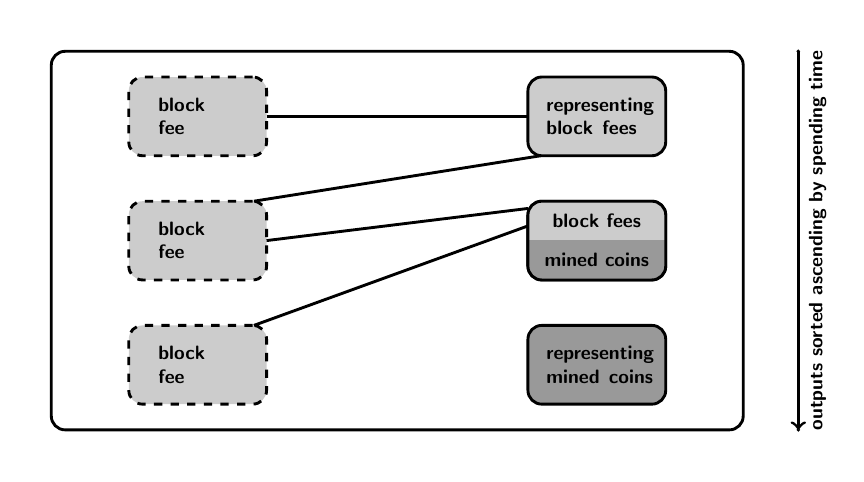
\begin{tikzpicture}[scale=1.0]
	\def \debugPoint   {}%
%	\def \debugPoint   {point}%
	\def \debugPointF  {point}%
	% font settings ############################################################
	\def \fontset      {\scriptsize\sffamily\bfseries}
	% color definition #########################################################
%	\def \colorOut     {jwigreige!50}
%	\def \colorOutH    {jwigreige!25!black}
	\def \colorIn      {black!10!white}
	\def \colorCoin    {white}
	\def \colorCoinY   {jwilightgreen!80!bg}
	\def \colorCoinN   {jwiorange}
	\def \colorCoinUtxoL {black!30!white}
	\def \colorCoinUtxo  {black!40!white}
	% arrow and line definitions ###############################################
	\def \lineW        {1.3pt}
	% width/height definition ##################################################
	\def \picW         {\columnwidth*24/31}%
	\def \picH         {\paperheight*6/31}%
	\def \TDX          {0.3cm}%
	\def \TDY          {0.3cm}%
	
	\def \IPosX        {\picW*3/10}%
	\def \IPosY        {\picH*7/24}%
	
	\def \SPosX        {0.7cm} % sorting position
	
	% tikz styles################################################################
	\tikzstyle{lineIO}       = [
		- ,
		line width = \lineW*0.8,
	]
	\tikzstyle{nodeOuter}    = [
%		draw,
%		rectangle,
%		rounded corners=5pt,
%		solid,
%		line width = \lineW,
%		black,
%		fill=\colorOut,
%		inner sep = 0pt,
%		outer sep = 0pt,
%		text width = \BOW,
%		minimum width = \BOW,
%		minimum height = \BOH*1.075,
		lineIO, 
		solid, 
		%		fill = black!20!white, 
		rounded corners=5pt
	]
	\tikzstyle{nodeInner}    = [
		draw,
		black,
		solid,
		rectangle,
		rounded corners=5pt,
		fill=black!20!white,
		minimum height = 1.0cm,
		minimum width = 1.75cm,
		text width = 1cm,
		lineIO,
		inner sep = 0pt,
		outer sep = 0pt,
	]	
	% coordinates ###############################################################
	% 1 | 2 | 3 | 4 | 5 | 6 | 7 | 8 | 9 | 10 | 11 | 12 | 13 | 14 |
	% A | B | C | D | E | F | G | H | I |  J |  K |  L |  M |  N |
	
	\coordinate (cen)    at ($( 0.0, 0.0) + ( 0.0        , 0.0         )$) (cen)   [\debugPoint];%
	\coordinate (Tcen)   at ($(cen)       + (-\picW*0.25 , 0.0         )$) (cen)   [\debugPoint];%
	
	\coordinate (PLU)    at ($(Tcen)      + (-\picW*0.5  , \picH*0.5   )$) (PLU)   [\debugPoint];%
	\coordinate (PLD)    at ($(Tcen)      + (-\picW*0.5  ,-\picH*0.5   )$) (PLD)   [\debugPoint];%
	\coordinate (PRU)    at ($(Tcen)      + ( \picW*0.5  , \picH*0.5   )$) (PRU)   [\debugPoint];%
	\coordinate (PRD)    at ($(Tcen)      + ( \picW*0.5  ,-\picH*0.5   )$) (PRD)   [\debugPoint];%
	
	\coordinate (TLU)    at ($(PLU)       + ( \TDX*1.0   ,-\TDY*1.0    )$) (TLU)   [\debugPoint];%
	\coordinate (TLD)    at ($(PLD)       + ( \TDX*1.0   , \TDY*1.0    )$) (TLD)   [\debugPoint];%
	\coordinate (TRU)    at ($(PRU)       + (-\TDX*1.0   ,-\TDY*1.0    )$) (TRU)   [\debugPoint];%
	\coordinate (TRD)    at ($(PRD)       + (-\TDX*1.0   , \TDY*1.0    )$) (TRD)   [\debugPoint];%
		
	\coordinate (IA)     at ($(Tcen)      + (-\IPosX*0.9 , \IPosY*1.0  )$) (IA)    [\debugPoint];%
	\coordinate (IB)     at ($(Tcen)      + (-\IPosX*0.9 , \IPosY*0.0  )$) (IB)    [\debugPoint];%
	\coordinate (IC)     at ($(Tcen)      + (-\IPosX*0.9 ,-\IPosY*1.0  )$) (IC)    [\debugPoint];%
	
	\coordinate (OA)     at ($(Tcen)      + ( \IPosX*0.9 , \IPosY*1.0  )$) (OA)    [\debugPoint];%
	\coordinate (OB)     at ($(Tcen)      + ( \IPosX*0.9 , \IPosY*0.0  )$) (OB)    [\debugPoint];%
	\coordinate (OC)     at ($(Tcen)      + ( \IPosX*0.9 ,-\IPosY*1.0  )$) (OC)    [\debugPoint];%
	
	%for sorting arrow
	\coordinate (SU)     at ($(TRU)       + ( \SPosX*1.0 , 0.0         )$) (SU)    [\debugPointF];%
	\coordinate (SD)     at ($(TRD)       + ( \SPosX*1.0 , 0.0         )$) (SD)    [\debugPointF];%
	
	%clipping
%	\clip ($(PLD) + ( 0.0 , 0.0)$) rectangle ($(PRU) + ( 0.0 ,-0.1)$);
	%basic picture
	
	% Slide numbering helper
	
%	\node[,] () at ($(cen) + ( 0.00, 0.00)$) {\fontset{}\large\textbf{1}};
%	\node[,] () at ($(cen) + ( 0.00, 0.00)$) {\fontset{}\large\textbf{2}};	
%	\node[,] () at ($(cen) + ( 0.00, 0.00)$) {\fontset{}\large\textbf{3}};
%	\node[,] () at ($(cen) + ( 0.00, 0.00)$) {\fontset{}\large\textbf{4}};
%	\node[,] () at ($(cen) + ( 0.00, 0.00)$) {\fontset{}\large\textbf{5}};
%	\node[,] () at ($(cen) + ( 0.00, 0.00)$) {\fontset{}\large\textbf{6}};
%	\node[,] () at ($(cen) + ( 0.00, 0.00)$) {\fontset{}\large\textbf{7}};
%	\node[,] () at ($(cen) + ( 0.00, 0.00)$) {\fontset{}\large\textbf{8}};
							
	%Vertical Lines============================================================%
	
	%Nodes=====================================================================%	
%	fill=black!20!white,
	\linespread{0.7}
	\draw[nodeOuter] (TLD) -- (TLU) -- (TRU) -- (TRD) -- cycle;
	%fee nodes as "inputs"
	\node[nodeInner, dashed](NIA) at (IA) {\fontset{}block fee};
	\node[nodeInner, dashed](NIB) at (IB) {\fontset{}block fee};
	\node[nodeInner, dashed](NIC) at (IC) {\fontset{}block fee};
	%outputs nodes, fee only node
	\node[nodeInner](NOA) at (OA) {};
	\node[nodeInner, draw=none, fill=none, align=left](NOAT) at ($(NOA.center) + (-4pt, 0pt)$) {\fontset{}representing\\\fontset{}\mbox{block fees}};
	%outputs nodes, partly fee/coins node
	\node[nodeInner,fill=none](NOB)  at (OB) {};
	\filldraw[black!20!white] (NOB.180) [rounded corners=5pt] -- (NOB.north west) -- (NOB.north east) -- (NOB.0) -- cycle;
	\filldraw[black!20!white] (NOB.180)  -- (NOB.170) -- (NOB.10) -- (NOB.0) -- cycle;
	\filldraw[black!40!white] (NOB.180) [rounded corners=5pt] -- (NOB.south west) -- (NOB.south east) -- (NOB.0) -- cycle;
	%coin only node
	\filldraw[black!40!white] (NOB.180)  -- (NOB.190) -- (NOB.350) -- (NOB.0) -- cycle;
	\node[nodeInner,fill=none](NOBB) at (OB) {};
	
	\node[ draw=none, fill=none](NOBTA) at ($(NOB.center) + (0pt, 0.25cm)$) {\fontset{}\mbox{block fees}};
	\node[ draw=none, fill=none](NOBTB) at ($(NOB.center) + (0pt,-0.25cm)$) {\fontset{}\mbox{mined coins}};
	\node[nodeInner,fill=black!40!white,](NOC) at (OC) {};
	\node[nodeInner, draw=none, fill=none](NOCT) at ($(NOC.center) + (-4pt, 0.00)$) {\fontset{}representing\\\fontset{}\mbox{mined coins}};
	
	%Arrows depending on nodes=================================================%
	\draw[lineIO,] (NIA.00) .. controls ($(NIA.00) + ( 0.00, 0.00)$) and ($(NOA.180) + ( 0.00, 0.00)$) .. (NOA.180);
	\draw[lineIO,] (NIB.35) .. controls ($(NIB.35) + ( 0.00, 0.00)$) and ($(NOA.215) + ( 0.00, 0.00)$) .. (NOA.215);
	\draw[lineIO,] (NIB.00) .. controls ($(NIB.00) + ( 0.00, 0.00)$) and ($(NOB.155) + ( 0.00, 0.00)$) .. (NOB.155);
	\draw[lineIO,] (NIC.35) .. controls ($(NIC.35) + ( 0.00, 0.00)$) and ($(NOB.168) + ( 0.00, 0.00)$) .. (NOB.168);
	
	\draw[lineIO, solid, ->] (SU) -- node [below, rotate=90] {\fontset{}outputs sorted ascending by spending time} (SD);
	
	%Coin Symbols==============================================================%
	%TxA-----------------------------------------------------------------------%
%	\pic[ ,] () at ($(NBAUBL.east) + (-\BOH*0.125,-\BOH*0.0375)$) {coin={0.7pt}{0.05}{\BOH*0.12}{\colorCoin} {black!80!white}{black!90!white}};

	
	%Counter Node==============================================================%
%	\pic[  ] ()        at ($(BCount) + ( \BOH*0.225/2, 0.05)$) {coin={1.0pt}{0.07}{\BOH*0.225}{\colorCoinY}{black!90!white}{black!100!white}};
\end{tikzpicture}
%}%
	\centering
	\caption{Overview of preprocessing of coinbase transactions. Although coinbase transactions have no inputs, we regard fees collected in a coinbase transactions's block as pseudo-inputs.}
\end{figure}



\subsection{Efficiency improvements}
\label{sec:novel_impl}%

\subsubsection{Intuition}
\label{sec:novel_impl_intuition}%
Our approach allows for reusing and adjusting information of calculations for prior time-windows instead of recalculating them entirely for every day. %
While the novel implementation allows effectively for larger time-windows \(\wndwLength\), we reuse the general approach for measuring money in circulation proposed in \cite{pernice2019cryptocurrencies}. %
We do adapt it, however, by adjusting and recombining its elements. %
Our implementation steps through time by iteration periods \(\iterp\) which we chose to be 1 day each. %
A single inductive step \(\iteri\) takes the amount of money in circulation for time window \(\wndw_\iteri\) and reuses most of its information to calculate an estimate for \(\wndw_{iteri+1}\). %
Simply put, for every iteration step we thus add a new day to \(\wndw_{\iteri}\) (lets call him \(d\)) and eliminate the oldest one (lets call him \(d_{sub}\)). %
As a consequence we have to adjust the estimate for window \(\wndw_\iteri\) for the transactions in the above two days. %
Roughly spoken, we thus:
\begin{enumerate}
\item add the value of monetary units put into circulation by the transactions of the day that was just added, %
\item and subtract monetary units that had belonged to the day that was just eliminated %
\end{enumerate}
from window \(\wndw_{\iteri}\) to form the new window \(\wndw_{\iteri+1}\). %
How do the two steps proceed exactly and why is that the same as looping over all transactions in period \(\wndw\) for which money in circulation is to be estimated?
Figure \ref{fig:aggr} illustrates the intuition. % 
While step 1 simply estimating, aggregating and lastly add money put to circulation for each transaction pursued in day \(d\) following the scheme in Section \ref{sec:orig_approach}, step 2 is slightly more complex. %
Simply subtracting aggregating money put into circulation by transactions during the eliminated day \(d_{sub}\) is inaccurate. %
While the respective transactions are to be eliminated from the information set of the new window \(\wndw_{\iteri+1}\), transactions within the window might be linked to outputs from transactions having occurred during the eliminated day. %
Thus those transactions, now linking to outputs generated before the shifted starting date of \(\wndw_{\iteri+1}\) are not respending outputs anymore but now are to be counted as putting money into circulation. %
\textbf{TODO: Link better to illustration when fig finished.}


Why are we relying on induction instead of simply pre-calculating estimates for each day separately and then aggregating them? %
\textbf{TODO: Add in what broke initial idea.}


\subsubsection{Algorithmic implementation}
\label{sec:novel_impl_algo}%
\textbf{[TODO: Here the variables are still not in line with the rest of the paper and window length, index and period confusing.]}

The sketched implementation of the inductive framework is given in Algorithm \ref{algo:code_aggr}. %
The framework takes window \(\wndw\) and pre-cashed a data structure offering the set of coinbase outputs representing fees per block-height as input. %
It then loops trough every iteration period \(d\) constituting the whole history of the blockchain. %
In a first preparative step, pre-computes helper-structures for each day \(d\):
\begin{itemize}
\item \( \MSetCirc_{1}[d] \), money drawn into active circulation by the transactions of day \( d \) if a window of 1 is assumed,
\item \( \MSetCircLB[d] \), money drawn into active circulation by the transactions of day \(d\) if a window of w is assumed,
\item \( \MSetCircLA[d] \), and a corrective value based on transaction outputs from transactions during day \(d\) that can no longer be seen as ``respent-coins'' for window \(\wndw\).  
\end{itemize}

For now, we will simply treat the above three structures as black boxes and focus on the iterative framework which starts at line 17 of the pseudo-code.%
\footnote{The calculations for the three helper-structure are summarized in the following paragraphs.} %

The regular inductive steps are taken for \(d \geq w \).%
\footnote{
For days \(d < \wndw \), money put into circulation for a window \(\wndw\) by transactions of day \(d\) is simply the output-sum of coinbase transactions \(\MSetCbs[d]\). %
We use this intuition to initialize the algorithm.} %
First of all, as described in Section \ref{sec:novel_impl_intuition}, we set \(\MSetCircAggr[d]\), money in circulation over time window \(w\) as measured for iteration day \(d\), simple to its last calculated value. %
This value is now the base for adjustments. %
Using the pre-computed values, we can simply following the intuition layed out in \ref{sec:novel_impl_intuition}: %
We add \(\MSetCircLB[d]\), and thus money brought into circulation on day \(d\) added to the previous window to \(\MSetCircAggr[d]\). %
After that, we then subtract money in circulation for the day eliminated from the \(\wndw - 1\) and thus \(\MSetCirc_{1}[d_{sub}]\). %
Without further adjustment, however, we would ignore that by shifting the window boundaries certain transaction outputs cannot be seen any longer as ``respent-coins'' as the spent output no longer lies ``inside'' the respectiv time window. %
We thus add \( \MSetCircLA[d_{sub}] \) which, roughly spoken, aggregates money brought into circulation by transactions sspending outputs of transactions during day \(d\) if the new window boundaries are applied. %

Why does this work?

\textbf{TODO: Plot with explanation}

How are \(\MSetCirc_{1}\), \( \MSetCircLA[d] \) and \( \MSetCircLB[d] \) calculated in detail? % 

As in the original implementation, the core of the estimation procedure is given by the decision rules determining the amount of money that is put into circulation by individual transactions (compare Algorithm \ref{algo:code_mcirc}).%
\footnote{Stressing the novel inductive implementation setup, we reduce the complexity of the calculations by illustrating only the calculations for the \ac{wba}. %
Note, that the pseudo-code for money in circulation under the assumptions of \ac{lifo} and \ac{fifo} can be checked out in our open-source repository \url{https://github.com/wiberlin/ccurr_velocity}.
}
If the respective amount can be estimated by looping trough all inputs \(\Inp_{t}\) of transaction \(t\) and adding up values of inputs \(\val(i)\) referencing to outputs of coinbase transactions or are generated before the first timestamp of time window \(\wndw\) which is characterizing the estimate to be achieved (compare Section \ref{sec:orig_approach}). %
This core-functionality is referenced as function throughout the paper as function \(GetMCirc\bigl(t,\,\typett,\,\wndw,\bigr)\). %

Let's first turn to the computation of \(\MSetCircLA[d]\) and \(\MSetCirc_{1}[d]\) respectively. %
Obviously, our implementation will just apply \(GetMCirc\bigl(t,\,\typett,\,\wndw,\bigr)\) to aggregate the money supply put into circulation by all transactions \(\TxD\) of day \(d\) that has been added when shifting the window in the inductive process. % 

The computation of adjustment value \(\MSetCircLB[d]\) is slightly more complex. %
As given in line 14 of Algorithm \ref{algo:code_aggr}, we apply a function \(\MCircAdj(t,w)\) to all transactions in day \(d\). %
The inner workings of \(\MCircAdj(t,w)\) are illustrated in Algorithm \ref{algo:code_outs_spent_within}: % 
For every transaction \(t\), \(\MCircAdj(t,w)\) loops through all outputs and establishes whether the respective output has served as input of a transaction within window \(\wndw\). %
For the output's ``spending-transacting'' we thus want to aggregate the values of outputs that represent money put into circulation with respect to the new window \(\wndw + 1\). %
In Algorithm \ref{algo:code_outs_spent_within}, this is illustrated by adding value of output 


% %%%%%%%%%%%%%%%%%%%%%%%%%%%%%%%%%%%%%%%%%%%%%%%%%%%%%%%%%%%%%%%%%%%%%
% %%%%% If confusion arises between "days forming iteration steps" and "days of measurement" 
% Assume that money in circulation with a look-back time window of length \(\wndwLength\) is to be estimated for day \(\perd\). %
% The helper-structure estimates how much money is been brought into active circulation during the period \([\iterp_{\Start},\iterp_{\End}]\): Before the events at day \(\iterp\), the respective money supply has remained untouched for \(\wndwLength\) days. With its transaction at day \(\iterp\), however, it can now be seen as circulating within period  \([\wndw_\Start\) to \(\wndw_\End]\). %
% While the helper-structure is estimating the value of monetary units which are ``activated'' by transactions of day \( \iterp \), it does neglect outputs which turn into ``already spent'' outputs in prior days within window \(\wndw\). %
% For example, in figure \ref{fig:mcirc_concept}, if we estimated the money supply for the period of iteration step \(\iterp\) we would count only money in circulation of 3 missing that transaction TX-C ``outside'' of period \(i\) activated a money supply of 2 with INP-1. %
% As a consequence it only coincides with the original estimator for the special case of \(\iterp % \wndw\). %

% While the original estimator requires the information of each transaction in time-window \(\wndw\), the helper-construct looks only at the transactions of iteration-step \(\iterp\) and checks their inputs age against \(\wndw_\Start\). % 

% The above helper-construct can be seen as the centerpiece to realize the inductive framework. %
% Algorithm \ref{algo:code_mcirc} offers a detailed summary. %
% %%%%%%%%%%%%%%%%%%%%%%%%%%%%%%%%%%%%%%%%%%%%%%%%%%%%%%%%%%%%%%%%%%%%%

\begin{figure}[ht!]%
	\centering
	\ifdefined\varInputFigs%
	%-------------------------------------------------------------------------------
\usetikzlibrary{calc}
%coordinate test point. Use as follows: 	\coordinate (cen) 	 	 at (0,0) (cen) [point];
\tikzset{
	every point/.style = {radius={\pgflinewidth}, opacity=1, draw, solid, fill=white},
	pt/.pic = {
		\begin{pgfonlayer}{foreground}
			\path[every point, #1] circle;
		\end{pgfonlayer}
	},
	point/.style={insert path={pic{pt={#1}}}}, point/.default={},
	point name/.style = {insert path={coordinate (#1)}}
}
%-------------------------------------------------------------------------------

% basic delacations
\pgfdeclarelayer{background}%
\pgfdeclarelayer{foreground}%
\pgfsetlayers{background,main,foreground}%

%Coin Symbol--------------------------------------------------------------------
\tikzset{%
	pics/coin/.style n args={3}{%
		code ={
			\def \coinLineWidth {#1}%
			\def \coinCenDist   {#2}%
			\def \circRad       {#3}%
			\def \signRad       {\circRad*0.20}%
			\def \signRadProp   {0.45}
			\def \signRadExt    {\signRad*\signRadProp}
			\def \signRadOut    {\signRad+\signRadExt}
			\def \signAngle     {30}
			\def \sinSignAngle  {sin(\signAngle)}
			\def \cosSignAngle  {cos(\signAngle)}
			\def \signWidth     {{pow((pow(\signRadOut,2)-pow(\sinSignAngle*\signRad,2)),0.5)-(\cosSignAngle)*\signRad)}}
			
			\def \startIX       {{cos(\signAngle)*\signRad}}
			\def \startIY       {{\sinSignAngle*\signRad}}
			
			\def \startOY       {\startIY}
			\def \signAngleOutS {{atan((\sinSignAngle*\signRad)/pow((pow(\signRadOut,2)-pow(\sinSignAngle*\signRad,2)),0.5))}}
			\def \signAngleOutE {{360-atan((\sinSignAngle*\signRad)/pow((pow(\signRadOut,2)-pow(\sinSignAngle*\signRad,2)),0.5))}}
	%
			\coordinate ()          at ( 0.0     , 0.0);%
			\coordinate (cen)       at ( 0.0     , 0.0);%
			\coordinate (cenB)      at ($(cen)    + ( 0.00,-\coinCenDist)$);%
						
			\node[
				circle,
				draw = black,
				fill = white,
				line width = \coinLineWidth,
				minimum size = \circRad,
				inner sep = 0pt,
				outer sep = 0pt,
			](NCD) at (cenB) {};
			
			\node[
				circle,
				draw = black,
				fill = white,
				line width = \coinLineWidth,
				minimum size = \circRad,
				inner sep = 0pt,
				outer sep = 0pt,
			](NCU) at (cen) {};
			
%			\draw[ - , line width = \coinLineWidth, black] (NCU.195) -- (NCD.195);
			\draw[-, line width = \coinLineWidth, black] (NCU.210) -- (NCD.210);
			\draw[-, line width = \coinLineWidth, black] (NCU.225) -- (NCD.225);
			\draw[-, line width = \coinLineWidth, black] (NCU.240) -- (NCD.240);
			\draw[-, line width = \coinLineWidth, black] (NCU.255) -- (NCD.255);
			\draw[-, line width = \coinLineWidth, black] (NCU.270) -- (NCD.270);
			\draw[-, line width = \coinLineWidth, black] (NCU.285) -- (NCD.285);
			\draw[-, line width = \coinLineWidth, black] (NCU.300) -- (NCD.300);
			\draw[-, line width = \coinLineWidth, black] (NCU.315) -- (NCD.315);
			\draw[-, line width = \coinLineWidth, black] (NCU.330) -- (NCD.330);
%			\draw[ - , line width = \coinLineWidth, black] (NCU.345) -- (NCD.345);
			
			\draw[
				 - ,
				 line width = \coinLineWidth,
				 black!80!white,
				 fill = black!80!white
			]
				(\startIX,-\startIY) arc (360-\signAngle:\signAngle:\signRad)
				-- +(\signWidth, 0.0)
				arc (\signAngleOutS:\signAngleOutE:\signRadOut)
				-- (\startIX,-\startIY)
				-- cycle
				;
		}%
		
	} ,%
	pics/coin/.default={1.0pt}{0.1}{1cm}%
}%
%
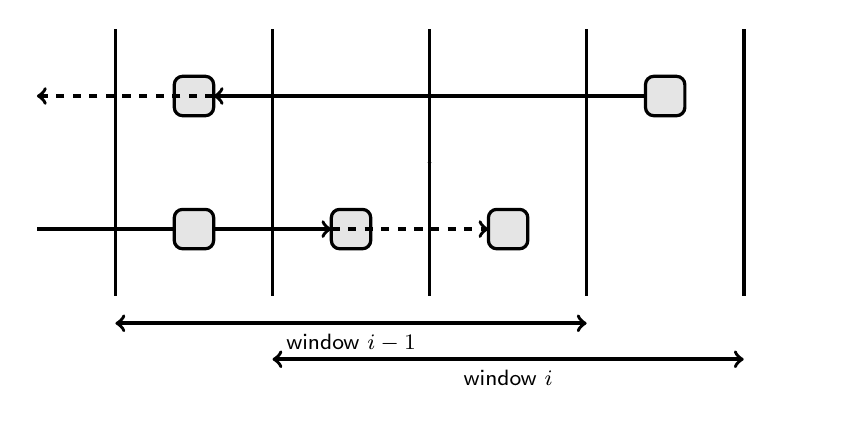
\begin{tikzpicture}
	\def \debugPoint   {}%
%	\def \debugPoint   {point}%
	\def \debugPointF  {point}%
	% font settings ############################################################
	\def \fontset      {\scriptsize\sffamily}
	\def \fontsetB     {\footnotesize\sffamily}
	% color definition #########################################################
	\def \colorOut     {black!100!white}
	\def \colorIn      {black!10!white}
	% arrow and line definitions ###############################################
	\def \lineW        {1.3pt}
	% width/height definition ##################################################
	\def \picW         {\columnwidth*25.5/31}%
	\def \picH         {\paperheight*3.75/31}%
	\def \TH           {\picH*0.4}%picH*0.5*0.8

	\def \DayD         {\picW*1/10}
	\def \BorD         {1em}

	% tikz styles################################################################
	\tikzstyle{lineIO} = [
		- ,
		line width = \lineW*0.8,
	]
	\tikzstyle{nodeOuter}   = [
		draw,
		rectangle,
		rounded corners=5pt,
		solid,
		line width = \lineW,
		black,
		inner sep = 0pt,
		outer sep = 0pt,
		text width = \BOW,
		minimum width = \BOW,
		minimum height = \BOH*1.075,
	]
	\tikzstyle{nodeInner}   = [
		draw,
		rectangle,
		rounded corners=3pt,
		solid,
		line width = \lineW*0.9,
		black,
		fill = \colorIn,
		inner sep = 0pt,
		outer sep = 0pt,
		align = center,
		text width = 0.5cm,
		minimum width = 0.5cm,
		minimum height = 0.5cm,
	]
	% coordinates ###############################################################
	% 1 | 2 | 3 | 4 | 5 | 6 | 7 | 8 | 9 | 10 | 11 | 12 | 13 | 14 |
	% A | B | C | D | E | F | G | H | I |  J |  K |  L |  M |  N |

	\coordinate (cen)       at ($(0.0,0.0)   + ( 0.0       , 0.0         )$) (cen)   [\debugPoint];%

	\coordinate (PLU)       at ($(cen)       + (-\picW*0.5 , \picH*0.5   )$) (PLU)   [\debugPoint];%
	\coordinate (PLD)       at ($(cen)       + (-\picW*0.5 ,-\picH*0.5   )$) (PLD)   [\debugPoint];%
	\coordinate (PRU)       at ($(cen)       + ( \picW*0.5 , \picH*0.5   )$) (PRU)   [\debugPoint];%
	\coordinate (PRD)       at ($(cen)       + ( \picW*0.5 ,-\picH*0.5   )$) (PRD)   [\debugPoint];%

	\coordinate (BCU)       at ($(cen)       + ( \picW*0.0 , \picH*0.5   )$) (BCU)   [\debugPoint];%
	\coordinate (BCD)       at ($(cen)       + ( \picW*0.0 ,-\picH*0.5   )$) (BCD)   [\debugPoint];%

	\coordinate (BLAU)      at ($(cen)       + (-\DayD*1.0 , \picH*0.5   )$) (BLAU)  [\debugPoint];%
	\coordinate (BLAD)      at ($(cen)       + (-\DayD*1.0 ,-\picH*0.5   )$) (BLAD)  [\debugPoint];%
	\coordinate (BLADD)     at ($(BLAD)      + ( 0.0       ,-\BorD*1.0   )$) (BLADD) [\debugPoint];%
	\coordinate (BLBU)      at ($(cen)       + (-\DayD*2.0 , \picH*0.5   )$) (BLBU)  [\debugPoint];%
	\coordinate (BLBD)      at ($(cen)       + (-\DayD*2.0 ,-\picH*0.5   )$) (BLBD)  [\debugPoint];%
	\coordinate (BLBDD)     at ($(BLBD)      + ( 0.0       ,-\BorD*1.0   )$) (BLBDD) [\debugPoint];%
	\coordinate (BLCU)      at ($(cen)       + (-\DayD*3.0 , \picH*0.5   )$) (BLCU)  [\debugPoint];%
	\coordinate (BLCD)      at ($(cen)       + (-\DayD*3.0 ,-\picH*0.5   )$) (BLCD)  [\debugPoint];%
	\coordinate (BLCDD)     at ($(BLCD)      + ( 0.0       ,-\BorD*1.0   )$) (BLCDD) [\debugPoint];%
	\coordinate (BLDU)      at ($(cen)       + (-\DayD*4.0 , \picH*0.5   )$) (BLDU)  [\debugPoint];%
	\coordinate (BLDD)      at ($(cen)       + (-\DayD*4.0 ,-\picH*0.5   )$) (BLDD)  [\debugPoint];%
	\coordinate (BLDDD)     at ($(BLDD)      + ( 0.0       ,-\BorD*1.0   )$) (BLDDD) [\debugPoint];%
%	\coordinate (BLEU)      at ($(cen)       + (-\DayD*4.5 , \picH*0.5   )$) (BLEU)  [\debugPoint];%
%	\coordinate (BLED)      at ($(cen)       + (-\DayD*4.5 ,-\picH*0.5   )$) (BLED)  [\debugPoint];%

	\coordinate (BRAU)      at ($(cen)       + ( \DayD*1.0 , \picH*0.5   )$) (BRAU)  [\debugPoint];%
	\coordinate (BRAD)      at ($(cen)       + ( \DayD*1.0 ,-\picH*0.5   )$) (BRAD)  [\debugPoint];%
	\coordinate (BRADD)     at ($(BRAD)      + ( 0.0       ,-\BorD*1.0   )$) (BRADD) [\debugPoint];%
	\coordinate (BRBU)      at ($(cen)       + ( \DayD*2.0 , \picH*0.5   )$) (BRBU)  [\debugPoint];%
	\coordinate (BRBD)      at ($(cen)       + ( \DayD*2.0 ,-\picH*0.5   )$) (BRBD)  [\debugPoint];%
	\coordinate (BRBDD)     at ($(BRBD)      + ( 0.0       ,-\BorD*1.0   )$) (BRBDD) [\debugPoint];%
	\coordinate (BRCU)      at ($(cen)       + ( \DayD*3.0 , \picH*0.5   )$) (BRCU)  [\debugPoint];%
	\coordinate (BRCD)      at ($(cen)       + ( \DayD*3.0 ,-\picH*0.5   )$) (BRCD)  [\debugPoint];%
	\coordinate (BRCDD)     at ($(BRCD)      + ( 0.0       ,-\BorD*1.0   )$) (BRCDD) [\debugPoint];%
	\coordinate (BRDU)      at ($(cen)       + ( \DayD*4.0 , \picH*0.5   )$) (BRDU)  [\debugPoint];%
	\coordinate (BRDD)      at ($(cen)       + ( \DayD*4.0 ,-\picH*0.5   )$) (BRDD)  [\debugPoint];%
	\coordinate (BRDDD)     at ($(BRDD)      + ( 0.0       ,-\BorD*1.0   )$) (BRDDD) [\debugPoint];%
%	\coordinate (BLDU)      at ($(cen)       + ( \DayD*4.5 , \picH*0.5   )$) (BLDU)  [\debugPoint];%
%	\coordinate (BLDD)      at ($(cen)       + ( \DayD*4.5 ,-\picH*0.5   )$) (BLDD)  [\debugPoint];%

	%clipping
%	\clip ($(PLD) + ( 0.0 ,-0.5)$) rectangle ($(PRU) + ( 0.0 , 0.1)$);
	%basic picture

	\draw[<->, solid, line width =\lineW] (BLDDD) -- node [midway, below] {\fontsetB{}window $i-1$} (BRBDD);
	\draw[<->, solid, line width =\lineW] ($(BLBDD) + ( 0.0,-\BorD*1.3)$) -- node [midway, below] {\fontsetB{}window $i$} ($(BRDDD) + ( 0.0,-\BorD*1.3)$);

	\draw[ -, solid , line width = \lineW] (BCU)   -- (BCD);
	\draw[ -, solid , line width = \lineW] (BLBU)  -- (BLBD);
	\draw[ -, solid , line width = \lineW] (BLDU)  -- (BLDD);
	\draw[ -, solid , line width = \lineW] (BRBU)  -- (BRBD);
	\draw[ -, solid , line width = \lineW] (BRDU)  -- (BRDD);

	%Nodes
	\node[nodeInner] (NRCA) at ($(BRCU)!0.25!(BRCD)$) {};
	\node[nodeInner] (NLCA) at ($(BLCU)!0.25!(BLCD)$) {};
	\node[point]     (NLEA) at ($(PLU)!0.25!(PLD)$) {};


	\node[nodeInner] (NLCB) at ($(BLCU)!0.75!(BLCD)$) {};
	\node[]          (NLEB) at ($(PLU)!0.75!(PLD)$) {};
	\node[nodeInner] (NLAB) at ($(BLAU)!0.75!(BLAD)$) {};
	\node[nodeInner] (NRAB) at ($(BRAU)!0.75!(BRAD)$) {};

	%Arrows depending on nodes
	\draw[ ->, line width = \lineW] (NRCA.west) -- (NLCA.east);
	\draw[ ->, line width = \lineW, dashed] (NLCA.east) -- (NLEA.center);

	\draw[ - , line width = \lineW] (NLCB.west) -- (NLEB.center);
	\draw[ ->, line width = \lineW] (NLCB.east) -- (NLAB.west);
	\draw[ ->, line width = \lineW, dashed] (NLAB.west) -- (NRAB.west);
\end{tikzpicture} 
	\else%
	\fi%
	\caption{%
		Overview of inductive computation of $\MCirc$. %
	}%
	\label{fig:aggr}%
\end{figure}%


%%% Local Variables:
%%% mode: latex
%%% TeX-master: "../main.tex"
%%% End:

